We report results across 18 two-agent backbone$\times$domain$\times$topology configurations. The central question: does communicative function predict which messages can be safely removed?

\subsection{Impact Gradient}
\label{sec:impact_gradient}

Figure~\ref{fig:impact}a shows the perturbation impact gradient: acknowledgments are the most locally disruptive yet informationally empty message type. Single-message removal disrupts 91\% of trajectories (mean similarity $= 0.352$), yet acknowledgments carry near-zero novel content (Qwen: 5.7\% bigram novelty, median 4 tokens; Appendix~\ref{app:info_theory}). Figure~\ref{fig:impact}b previews the resolution: despite high local sensitivity, cumulative type elimination shows that ack removal preserves accuracy (detailed in \S\ref{sec:e2e_pruning}).
A neutralize ablation confirms that disruption stems from conversational position, not content: replacement with a generic placeholder is more disruptive than outright deletion (similarity 0.196 vs.\ 0.352; $p < 0.001$; full per-type breakdown in Appendix~\ref{app:neutralize}). Llama acknowledgments exhibit an additional asymmetry: they never correct errors (0/1{,}483 messages) yet inject errors 14.3\% of the time (Appendix~\ref{app:info_theory}).

The impact gradient exhibits a clear separation: a likelihood-ratio test confirms that function type significantly predicts perturbation sensitivity ($\chi^2 = 47.3$, $p < 10^{-9}$; BH-corrected). Acknowledgments cluster tightly at low similarity (IQR $[0.18, 0.52]$), while information-provision and reasoning-guidance messages distribute broadly above 0.7, reflecting their variable contribution to task progress. In the forest plot (Figure~\ref{fig:forest}), all primary Qwen configurations fall within the $\pm 1$\,pp equivalence band, and the pooled 10-seed CI excludes effects larger than 1.13\,pp. Boundary conditions (MATH, Qwen3) produce CIs that extend below $-3$\,pp, confirming that the non-inferiority margin correctly flags unsafe configurations.

\begin{figure*}[t]
\centering
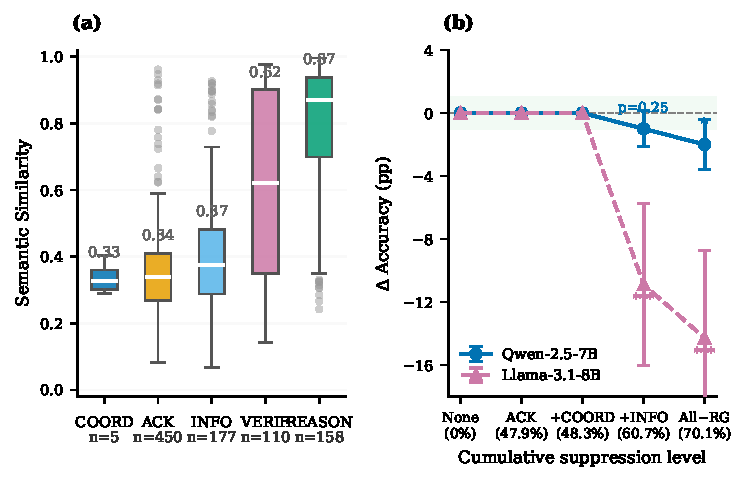
\includegraphics[width=\textwidth]{figures/figure2_combined.pdf}
\caption{(a)~Remove-ablation similarity by function type (Qwen2.5-7B, $n{=}895$). Lower $=$ greater disruption; acknowledgments (acks; median $= 0.34$) most impactful despite least information. The COORD boxplot ($n{=}5$) should be interpreted with caution given the small sample size. (b)~Cumulative type-elimination dose-response (None $\to$ ACK $\to$ +COORD $\to$ +INFO $\to$ All-RG). Qwen holds within 1\,pp through +INFO; only All-RG (70\% suppression) reaches significance. Llama drops sharply at +INFO (68\% suppression). Error bars: 95\% CIs from McNemar's discordant pairs.}
\label{fig:impact_and_dose}
\label{fig:impact}
\label{fig:dose_response}
\vspace{-6pt}
\end{figure*}

\subsection{E2E Communication Pruning}
\label{sec:e2e_pruning}

Despite high local sensitivity, bulk acknowledgment removal is safe. Both primary backbones meet non-inferiority at $\delta = -3$\,pp ($p < 0.001$; Table~\ref{tab:oracle_pruning}; Figure~\ref{fig:forest}). Qwen prunes 56\% of messages with near-zero accuracy change ($\Delta = +0.40 \pm 1.02$\,pp, 10 seeds; 95\% CI $[-0.33, +1.13]$\,pp). Llama prunes 36\% with a positive shift ($\Delta = +2.1 \pm 2.4$\,pp, 9/10 seeds positive), consistent with error-channel removal (\S\ref{sec:causal_injection}). Only boundary conditions (MATH, Qwen3) degrade (Appendix~\ref{app:boundary_conditions}).

\begin{table*}[t]
\centering
\caption{Oracle pruning accuracy (\%). GPT-4o ack-only detection. Multi-seed rows report mean$\pm$SD. Llama/StratQA: $N{=}238$ due to context overflow. Llama/GSM8K 10-seed: $N{=}1{,}939$ after filtering. Details: Appendix~\ref{app:online}.\protect\footnotemark}
\label{tab:oracle_pruning}
\small
\begin{tabular}{lcccr}
\toprule
\textbf{Setting} & $N$ & $\Delta$ \textbf{(pp)} & $p$ & \textbf{Supp.} \\
\midrule
Llama / GSM8K & 500 & $-0.6$ & .710 & 36.6\% \\
Qwen / GSM8K & 500 & $+0.8$ & .340 & 56.3\% \\
Qwen / GSM8K ($t{=}0.7$, 10s) & 10${\times}$200 & $+0.30 \pm 1.80$ & ${<}.001$\textsuperscript{$\ddagger$} & 39.2\% \\
Qwen / StratQA & 500 & $+0.2$ & 1.000 & 65.6\% \\
Llama / StratQA & 238 & $+5.0$ & .180 & 21.5\% \\
Qwen / ARC & \arcN{} & $\arcQwenDelta{}$ & \arcQwenPvalue{} & \arcQwenSupp{}\% \\
Qwen / GSM8K (10 seeds) & 10${\times}$200 & $+0.40 \pm 1.02$ & .048\textsuperscript{$\dagger$} & 56.0\% \\
Llama / GSM8K (10 seeds) & 10${\times}$200 & $+2.1 \pm 2.4$ & ${<}.001$\textsuperscript{$\ddagger$} & 36.5\% \\
\bottomrule
\end{tabular}
\end{table*}
\footnotetext{$^\dagger$TOST equivalence $\pm 1$\,pp (marginal); $^\ddagger$non-inferiority at $\delta = -3$\,pp.}

\begin{figure*}[t]
\centering
\includegraphics[width=\textwidth]{figures/figure3_forest.pdf}
\caption{Forest plot of pruning $\Delta$\,pp with 95\% CIs. Green band: $\pm 1$\,pp TOST equivalence; blue band: $-3$\,pp non-inferiority margin. Oracle and heuristic results cluster near zero for Qwen and Llama; boundary conditions (MATH, Qwen3) degrade beyond the non-inferiority margin.}
\label{fig:forest}
\end{figure*}

\begin{table*}[t]
\centering
\caption{Heuristic pruning accuracy (\%). Annotation-free detectors (F1\textsubscript{GSM8K} $= 0.845$/$0.805$). DistilBERT (F1 $= 0.867$) yields consistent results (Appendix~\ref{app:learned_classifier_details}).}
\label{tab:heuristic_pruning}
\small
\begin{tabular}{lcccr}
\toprule
\textbf{Setting} & $N$ & $\Delta$ \textbf{(pp)} & $p$ & \textbf{Supp.} \\
\midrule
Llama / GSM8K (5 seeds) & 5${\times}$200 & $+2.20 \pm 1.44$ & ${<}.001$\textsuperscript{$\ddagger$} & 74.9\% \\
Qwen / GSM8K (10 runs) & 10${\times}$200 & $-0.05 \pm 0.99$ & .880 & 41.8\% \\
Qwen / StratQA (5 seeds) & 5${\times}$200 & $+0.70 \pm 0.91$ & ${<}.001$\textsuperscript{$\ddagger$} & 56.9\% \\
Llama / StratQA (8 seeds) & 8${\times}$200 & $+2.81 \pm 3.94$ & .002\textsuperscript{$\ddagger$} & 50.3\% \\
Gemma / GSM8K$^\star$ & 300 & $+0.7$ & .683 & 79.3\% \\
\bottomrule
\end{tabular}
\\[2pt]
{\scriptsize $^\star$Exploratory; confounded: suppress rate (79.3\%) $\gg$ oracle ack rate ({$<$}5\%). $^\ddagger$Non-inferiority at $\delta = -3$\,pp.}
\end{table*}

\paragraph{Efficiency.} Each suppressed acknowledgment eliminates one full LLM generation call. Qwen achieves 56\% call reduction and ${\sim}$10.1\% token reduction; Llama achieves 36.5\% and ${\sim}$27.5\% respectively (oracle, GSM8K, 10 seeds). The disparity between Qwen's 56\% and Llama's 36.5\% call savings reflects their contrasting acknowledgment rates: Qwen produces short, formulaic confirmations at every checker turn (median 4 tokens, 56\% of all messages), whereas Llama generates verbose responses that the annotator less frequently classifies as pure acknowledgments. Token savings remain modest (10--28\%) because the eliminated messages are disproportionately short; a single reasoning-guidance message can exceed 100 tokens, which dwarfs the cumulative savings from several pruned acks. The practical benefit is therefore latency reduction rather than bandwidth savings: each pruned acknowledgment eliminates one full inference call with its associated scheduling and memory-allocation overhead (Appendix~\ref{app:efficiency}).

\paragraph{Heuristic and cross-domain safety.} Heuristic detectors achieve these savings at zero marginal cost; cross-domain (StratQA) results are consistent with non-inferiority (Table~\ref{tab:heuristic_pruning}). Qwen's heuristic serves as the primary annotation-free validation (suppress rate 41.8\%, consistent with the 56\% oracle ack rate). Llama's heuristic over-suppresses at 74.9\% (vs.\ 36.5\% oracle ack rate; only 32.9\% of suppressed messages are true acknowledgments), so its positive $\Delta$ constitutes a \emph{robustness upper bound}: if suppressing 75\% of messages---most not acknowledgments---produces no degradation, the conservative oracle ack-only pruning is a fortiori safe (Appendix~\ref{app:online}). For Qwen, pruning remains robust under stochastic sampling ($t{=}0.7$); Llama shows sensitivity from $t{\geq}0.3$ (Appendix~\ref{app:temp-robustness}). FG pruning degrades accuracy in exploratory comparison ($-5.0$\,pp vs.\ $+1.0$ for ack-only, $p = 0.031$; Appendix~\ref{app:statistical}), confirming that five-class sub-type distinctions add no incremental value over binary ack/non-ack for pruning decisions.

\paragraph{Scaling and generalization.} Safety holds across three detector types and extends beyond the primary 7B two-agent setting. At 72B scale, Qwen2.5-72B-Instruct-AWQ oracle pruning ($N{=}\qwenSevenTwoBN{}$, 5 seeds) yields $\Delta = \qwenSevenTwoBDelta{} \pm \qwenSevenTwoBSD{}$\,pp with TOST equivalence at $\pm 1$\,pp ($p = \qwenSevenTwoBPvalue{}$; Appendix~\ref{app:scaling}); ack rates at 14B (31.7\%) and 72B (\qwenSevenTwoBSupp{}\%) suggest scale-invariant communication structure. A 3-agent solver-checker-critic pilot (3 seeds, $N{=}100$ per seed) produces $\Delta = -0.67 \pm 0.29$\,pp, passing non-inferiority at $\delta = -3$\,pp ($p = 0.003$; Appendix~\ref{app:multiagent}), providing preliminary evidence that pruning generalizes from round-robin dyads to chain topologies.

\subsection{Injection Experiments Reveal Backbone-Dependent Mechanisms}
\label{sec:causal_injection}

Function predicts not only which messages to prune but why pruning works. Injection experiments (5-seed GSM8K, single-seed StratQA) and random-deletion controls jointly reveal a backbone-dependent dissociation.
Qwen acknowledgments are structurally redundant. We insert acknowledgments into non-ack positions and observe no detectable accuracy change on GSM8K ($\bar{\Delta} = -0.20$\,pp, $p = 0.71$, five seeds, $N \approx 300$ per seed) or StratQA ($p = 0.784$, $N = 250$; single seed). Inject or remove: Qwen performance is unchanged.

Llama acknowledgments function as an error channel. Injection significantly harms accuracy on GSM8K ($\bar{\Delta} = -3.88$\,pp, $\mathrm{SD} = 1.34$, $p = 0.0029$, five seeds, $N \approx 294$ per seed), with a directionally consistent trend on StratQA ($\Delta = -3.28$\,pp, $p = 0.271$, $N = 244$; single seed). The asymmetry is quantitatively stark (Figure~\ref{fig:injection}b): Llama's injection effect size ($h = 0.10$) exceeds Qwen's ($h < 0.01$) by an order of magnitude, and the cross-domain direction holds on StratQA despite reduced statistical power. Removal eliminates this error pathway, which explains the positive pruning shift in Table~\ref{tab:oracle_pruning}.

At these suppression rates, message-count-matched random deletion is equally harmless (Qwen$\times$GSM8K: $p = 0.724$; Llama$\times$GSM8K: $p = 0.831$). Ack-targeted pruning's value lies in automatic identifiability. The cumulative type-elimination curve (Figure~\ref{fig:impact}b) reveals that safety is function-specific at higher rates: random deletion at higher counts risks removing task-critical reasoning guidance. Function analysis identifies both the safe category and the safe quantity (token-matched control in Appendix~\ref{app:token_matched}).

The dose-response gradient constitutes causal evidence for function-type specificity: the taxonomy identifies the boundary between safe (ACK, COORD) and harmful suppression (INFO, reasoning guidance) at 68--70\% removal. These results resolve the opening paradox: local disruption does not predict functional necessity (\S\ref{sec:discussion}). \emph{Limitation:} StratQA injection uses a single seed; cross-seed replication for this domain remains future work.

\subsection{Cross-Domain Consistency}
\label{sec:cross_domain}

Backbone identity dominates communication patterns more than domain choice (Cram\'{e}r's $V = 0.45$~\citep{cramer_1946} vs.\ $0.18$ for domain). The cross-domain oracle matrix shows no significant accuracy drops (Table~\ref{tab:oracle_pruning}). Oracle pruning on ARC ($N{=}\arcN{}$) extends validation to a third domain (Qwen $\Delta = \arcQwenDelta{}$\,pp; Llama $\Delta = \arcLlamaDelta{}$\,pp, $p = \arcLlamaPvalue{}$). Two boundary conditions validate by counter-example: on MATH, acknowledgments carry substantive content and pruning degrades accuracy; on Qwen3-8B, heuristic over-suppression causes a 14\,pp drop (Appendix~\ref{app:boundary_conditions}). These failures confirm that pruning is safe precisely when acknowledgments are functionally redundant.

\subsection{Backbone Communication Typology}
\label{sec:three_modes}

Mixed-effects models ($N = 2{,}294$; Appendix~\ref{app:mixed-effects}) reveal three topology-stable profiles: \textbf{function-organized} (Qwen), \textbf{position-organized} (Gemma; exploratory, $\kappa = 0.35$, $< 5\%$ acks), and \textbf{undifferentiated} (Llama). Backbone $\times$ function\_type interaction is highly significant ($p < 10^{-41}$), stable across topologies ($p = 0.963$; per-topology breakdowns in Appendix~\ref{app:statistical}).
The function-organized profile (Qwen) concentrates 48\% of messages as acknowledgments (Table~\ref{tab:taxonomy}) with the highest inter-type variance in perturbation sensitivity (Levene's $F = 12.4$, $p < 0.001$), making function-targeted pruning most effective. The position-organized profile (Gemma) distributes 56\% as information provision regardless of dialogue position, produces fewer than 5\% acknowledgments, and shows minimal type differentiation in ablation response. The undifferentiated profile (Llama) distributes messages evenly yet exhibits a unique error-channel property where acknowledgments carry fabricated content.
\begin{figure*}[t]
\centering
\includegraphics[width=\textwidth]{figures/figure4_combined.pdf}
\caption{Backbone-dependent communication. (a)~Function type distribution by backbone (round-robin, GSM8K, $N{=}300$ each). Qwen and Llama concentrate $>$47\% of messages as acknowledgments; Gemma is dominated by information provision (56\%). (b)~Acknowledgment injection effect: inserting acks into non-ack positions is harmless for Qwen ($p = 0.71$, five seeds) but degrades Llama accuracy ($\bar{\Delta} = -3.88$\,pp, $p = 0.0029$, five seeds), revealing backbone-dependent mechanisms. Green band: $\pm 1$\,pp equivalence zone.}
\label{fig:distribution}
\label{fig:injection}
\vspace{-6pt}
\end{figure*}
